\subsection{Application: Precision Agriculture and Autonomous Farming}

Precision agriculture is a strong Foundations application because agricultural prediction depends heavily on representation, label quality, and validation design. A single vegetation index measured at one date can collapse seasonal information that separates crops, orchards, grassland, forest, water, and built surfaces. Conversely, a temporal feature representation can encode phenological change over the growing season without requiring a specialized deep sequence model. This makes the domain well suited for demonstrating how feature design changes the effective hypothesis space.

Agricultural data also illustrates the importance of dataset provenance. Crowdsourced labels can be noisy because field boundaries, land-cover categories, and acquisition dates are imperfectly observed. The benchmark used here explicitly distinguishes a noisy training file from a cleaner testing file, providing a concrete example of Chapter 1 topics such as label noise, distribution quality, validation discipline, and the need to avoid interpreting a test score without understanding how the labels were produced.

The reproduced experiment uses Landsat-derived normalized difference vegetation index (NDVI) features from the UCI Crowdsourced Mapping dataset. It compares a model that sees only the maximum NDVI value with models that use the complete dated NDVI sequence. The comparison is intentionally conventional: logistic regression isolates the effect of representation under a linear hypothesis class, while a random forest tests whether nonlinear interactions among acquisition dates add value.

\textbf{Problem}

The task is multiclass land-cover classification from remotely sensed vegetation measurements. The target classes are farm, forest, grass, impervious surface, orchard, and water. For precision-agriculture use, correct separation of farm and orchard classes is especially important, but macro-averaged metrics are also needed so that common classes do not dominate the evaluation.

\textbf{Dataset}

The benchmark uses the UCI Crowdsourced Mapping dataset (repository identifier 400). The predictors include maximum NDVI and 27 dated NDVI measurements spanning 2014--2015, for 28 NDVI features in total. The dataset documentation notes that the training labels contain errors, whereas the testing labels are intended as clean ground truth. That distinction is preserved rather than silently treating both partitions as equally reliable.

\textbf{Model}

Three models are compared. Max-NDVI logistic regression uses only the scalar maximum NDVI feature. NDVI-time-series logistic regression uses all 28 NDVI measurements, allowing a linear model to exploit seasonal profile information. The NDVI random forest uses the same 28 features but can model nonlinear interactions and threshold effects across acquisition dates.

\textbf{Method}

The supplied training file is used for fitting, and the supplied clean testing file is reserved for final evaluation. Logistic-regression predictors are standardized from the training data. No information from the testing labels is used for feature selection. The experiment reports overall accuracy together with macro-F1 because the six land-cover classes need not be equally represented.

\textbf{Evaluation}

Figure~\ref{fig:ch1-precision-agriculture} combines the temporal representation and the class-level diagnostic. Panel (a) shows the mean dated NDVI profile for each testing-set land-cover class, revealing that the temporal trajectories contain substantially more structure than a single maximum value. Panel (b) shows the row-normalized confusion matrix for the strongest reproduced model, with a quantitative colorbar from 0 to 1. Table~\ref{tab:ch1-precision-agriculture-benchmark} compares the three feature/model configurations.

\begin{figure}[t]
\centering
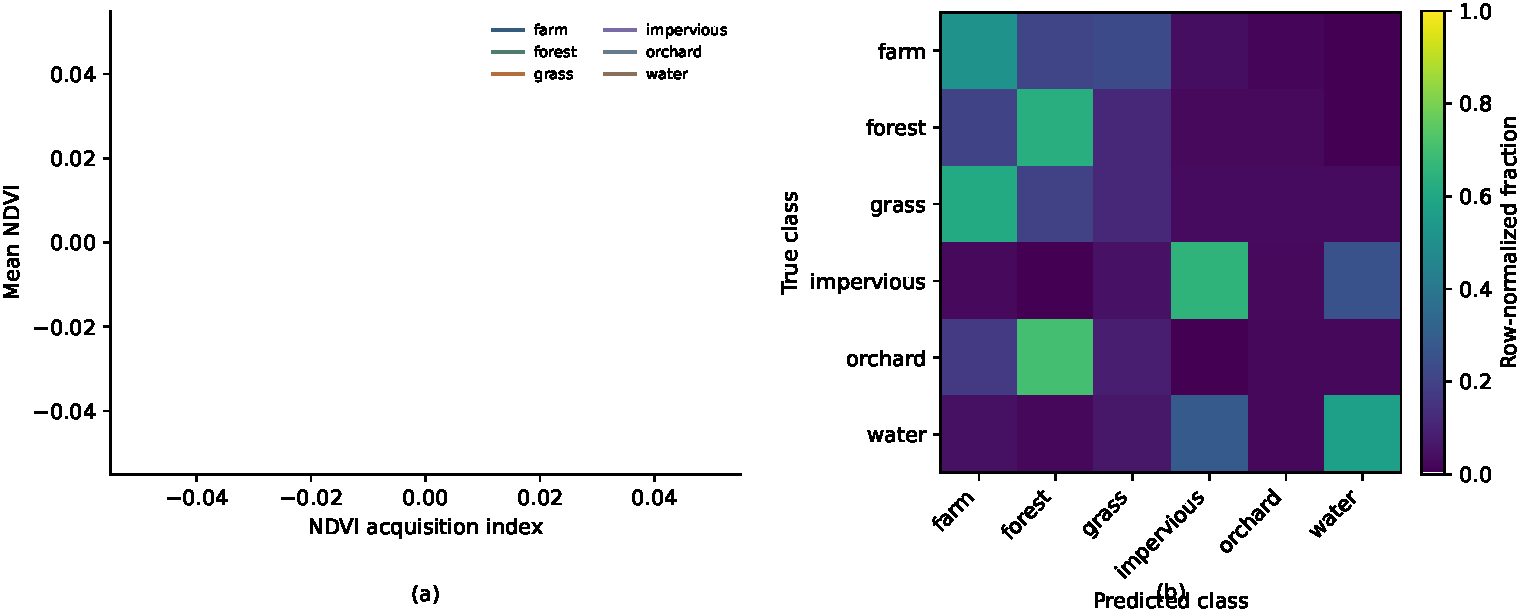
\includegraphics[width=\BookFigureWidth]{figures/ch01_precision_agriculture_ndvi.pdf}
\caption{Reproduced land-cover classification diagnostics from the UCI Crowdsourced Mapping dataset. (a) Mean NDVI trajectories across dated Landsat acquisitions for farm, forest, grass, impervious, orchard, and water classes. The seasonal profiles demonstrate information that is lost when the representation is reduced to a single maximum-NDVI scalar. (b) Row-normalized confusion matrix for the 28-feature NDVI random forest on the clean testing labels. The colorbar reports the fraction of examples within each true class assigned to each predicted class.}
\label{fig:ch1-precision-agriculture}
\end{figure}

\begin{table}[t]
\centering
\small
\caption{Reproduced UCI Crowdsourced Mapping benchmark comparing a scalar vegetation summary with the complete NDVI time-series representation. Macro-F1 weights the six land-cover classes equally.}
\label{tab:ch1-precision-agriculture-benchmark}
\begin{tabular}{lrrr}
\toprule
Model & Features & Accuracy & Macro-F1 \\
\midrule
Max-NDVI logistic & 1 & 0.410 & 0.248 \\
NDVI-time-series logistic & 28 & 0.630 & 0.608 \\
NDVI random forest & 28 & 0.690 & 0.664 \\
\bottomrule
\end{tabular}
\end{table}

\textbf{Results}

Replacing the single maximum-NDVI feature with the full 28-feature vegetation trajectory increases logistic-regression accuracy from 0.41 to 0.63 and macro-F1 from 0.248 to 0.608. The random forest improves further to 0.69 accuracy and 0.664 macro-F1. The comparison demonstrates two Chapter 1 ideas simultaneously: richer representation can make a simple model substantially more effective, and nonlinear interactions can add value once the informative temporal variables are preserved.

\textbf{Error Analysis}

The normalized confusion matrix should be examined class by class rather than reduced to overall accuracy. Farm, orchard, forest, and grass can exhibit overlapping seasonal vegetation profiles, while impervious surfaces and water are often easier to distinguish. Errors may reflect genuine spectral similarity, label noise in the training data, mixed pixels, temporal misregistration, or differences in crop calendar. Because the training labels are known to contain noise, some systematic errors may arise from supervision quality rather than model capacity.

\textbf{Limitations}

The benchmark is a land-cover mapping dataset rather than a complete autonomous-farming system. It does not include field-level management decisions, yield prediction, soil chemistry, weather forecasts, irrigation control, or robotic actuation. Spatial autocorrelation may also cause nearby observations to be more similar than independent random samples. A production agricultural study should therefore add spatially separated validation, explicit geographic provenance, and season-to-season holdouts.

\textbf{Deployment / Engineering Implications}

The Chapter 1 lesson is that agricultural ML should preserve the temporal and spatial information needed by the decision while treating label provenance as part of the statistical problem. A deployment pipeline should monitor seasonal shift, sensor calibration, cloud contamination, crop rotations, and changing field boundaries. Strong performance on one season or geography does not establish generalization to another, so geographic and temporal holdouts are essential before a model is used for agronomic decisions.
